\paragraph{Treść}~\\
Proszę odtworzyć wykres znajdujący się na \textit{rysunku}.

\begin{figure}[p]
  \caption{Rysunek załączony do zadania}
  \label{fig:TestowyPng}
  \centering
  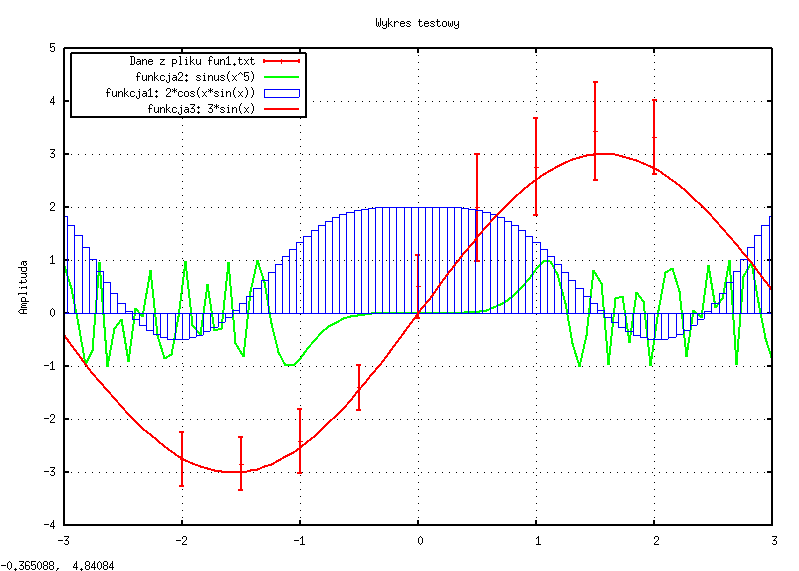
\includegraphics[width=\textwidth]{testowy.png}
\end{figure}

\lstinputlisting[caption=Zawartość pliku fun1.txt,label=lst:Fun1Txt]{fun1.txt}

\lstinputlisting[caption=Komendy dla programu gnuplot do zadania 3,label=lst:TestowyTxt]{testowy.txt}

\begin{figure}[p]
  \caption{Wynik programu gnuplot dla komend do zadania 3}
  \label{fig:TestowyJpg}
  \centering
  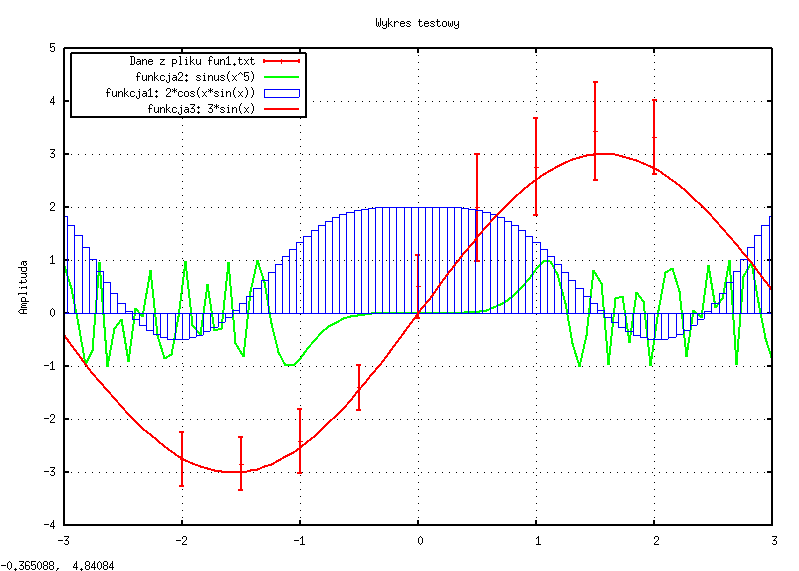
\includegraphics[width=\textwidth]{testowy.jpg}
\end{figure}

\paragraph{Podsumowanie}~\\
Wynik generowany jest poprzez załadowanie do programu gnuplot komend z listowania~\ref{lst:TestowyTxt}.
Komendy mają na zadanie odwzorować rysunek~\ref{fig:TestowyPng} załaczony do zadania.
Dane dla czerwonego wykresu zostały odczytane na podstawie załączonego obrazka i zapisane do pliku fun1.txt, którego zawartość widnieje na listowaniu~\ref{lst:Fun1Txt}.
Niestety, ze względu na słabą jakość obrazka źródłowego udało mi się odczytać przybliżone pojedyncze wartości, dlatego na wykresie są one zaznaczone jako punkty.
Wynik zaprezentowany został na rysunku~\ref{fig:TestowyJpg}.
